\documentclass{article}
\usepackage[UTF8]{ctex}
\usepackage{amsfonts}
\usepackage{amsmath}
\usepackage{float}
\usepackage{graphicx}
\usepackage{url}

\newcommand{\Bezier}{B\'ezier}%Bézier

\usepackage{color}

% paragraph
\setlength{\parindent}{1pt}
\setlength\parskip{\baselineskip}
\renewcommand{\baselinestretch}{1.2}

\begin{document}
	
	% 标题
	\title{《计算机辅助几何设计》作业}
	\author{ID号: 048  \qquad  姓名: 郑涛}  %递交作业时填上ID号和姓名
	\date{2024年10月26日}
	\maketitle

\section{问题描述}
	给定n+1个点$p_i(i=0,\dots,n)$,实现四阶三次B样条插值曲线$x(t)$以及交互功能。
\section{程序思路说明}
\subsection{De Boor Algorithm}
给定n+1个De Boor Points:$d_i(i=0,\dots,n)$,以及结点向量
$$(t_0=t_1=\cdots=t_{k-1},t_k,t_{k+1},\dots,t_{n+1}=t_{n+2}=\cdots=t_{n+k})$$
伪代码:
\begin{figure}[H]
	\flushleft
	\includegraphics[scale=0.5]{"De Boor Algorithm"}
	\label{fig:de-boor-algorithm}
\end{figure}

\subsection{如何实现四阶三次B样条曲线插值}
B样条曲线有形式:
	$$x(t)=\sum_{i=0}^{n}N_{i,k}(t)\cdot d_i$$
其中$N_{i,k}(t)$为B样条基函数,满足如下关系:
\begin{equation*}
	N_{i,1}(t)=
	\left\{
	\begin{aligned}
		&1,t_i\leq t\textless t_{i+1}\\
		&0,otherwise
	\end{aligned}
	\right.
\end{equation*}
\begin{equation*}
	\begin{aligned}
		N_{i,k}(t)=\frac{t-t_i}{t_{i+k-1}-t_i}N_{i,k-1}(t)&+\frac{t_{i+k}-t}{t_{i+k}-t_{i+1}}N_{i+1,k-1}(t)\\
		for\,k\textgreater1,&i=0,\dots,n
	\end{aligned}
\end{equation*}
四阶B样条插值函数的De Boor Points $d_i(i=0,1,\dots,n+2)$要满足:
\begin{enumerate}
	\item [1.]选定Knot Vector:
	\begin{equation}
		\begin{aligned}
			T&=(t_0,t_1,t_2,t_3,t_4,\dots,t_{n+2},t_{n+3},t_{n+4},t_{n+5},t_{n+6})\\
			&=(s_0,s_0,s_0,s_0,s_1,\dots,s_{n-1},s_n,s_n,s_n,s_n)
		\end{aligned}
	\end{equation}
	\item  [2.]满足插值条件:
	\begin{equation}
		\begin{aligned}
			x(s_0)&=p_0=d_0\\
			x(s_i)&=p_i=N_{i,4}(s_i)d_i+N_{i+1,4}(s_i)d_{i+1}+N_{i+2,4}(s_i)d_{i+2}\\
			x(s_n)&=p_n=d_{n+2}
		\end{aligned}
	\end{equation}
	\item [3.]上述有$n+1$个条件,要求$n+3$个De Boor Point,需要加两个条件:
	\begin{equation}
		\begin{aligned}
			x''(s_0)&=0\Leftrightarrow \frac{d_2-d_1}{s_2-s_0}=\frac{d_1-d_0}{s_1-s_0}\\
			x''(s_n)&=0\Leftrightarrow \frac{d_{n+2}-d_{n+1}}{s_n-s_{n-1}}=\frac{d_{n+1}-d_n}{s_n-s_{n-2}}
		\end{aligned}
	\end{equation}
\end{enumerate}
根据上述条件解线性方程组求出De Boor Points $d_i(i=0,1,\dots,n+2)$,再根据De Boor Algorithm求得B样条曲线即可。
\section{编译环境}
	本代码用matlab R2022b编译
\section{使用说明}
	本代码可直接运行,移动其中一点之后可以看到控制点和控制点的折线。
\section{结果展示}
	\begin{figure}[H]
		\centering
		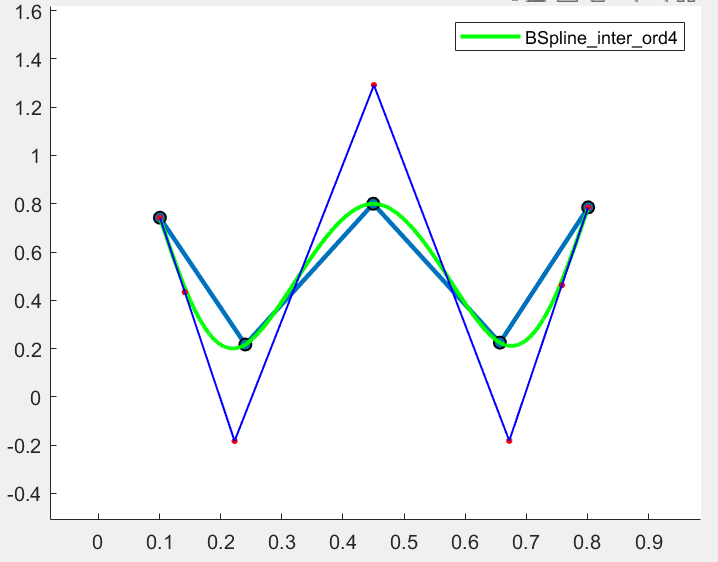
\includegraphics{w}
		\caption{}
		\label{fig:w}
	\end{figure}
	\begin{figure}[H]
		\centering
		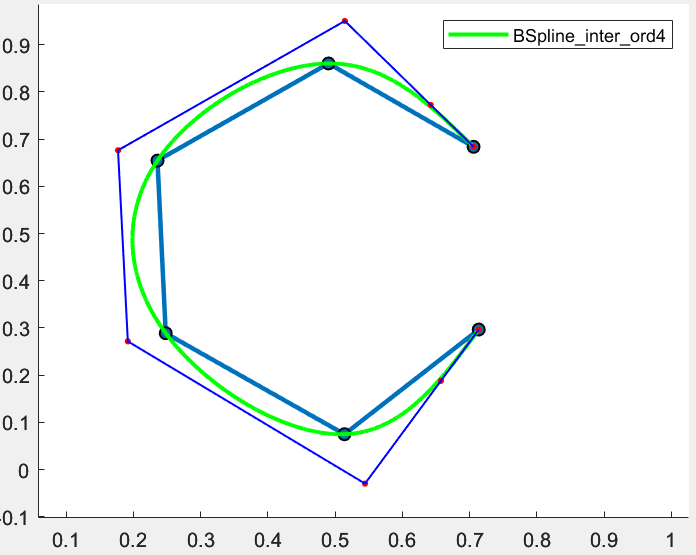
\includegraphics{c}
		\caption{}
		\label{fig:c}
	\end{figure}
\section{实验结果分析}
	实现了四阶三次B样条曲线插值以及交互功能。

\end{document}











